%Pretreatment========================================================================================
\documentclass[12pt]{article}
\usepackage{lingmacros}
\usepackage{tree-dvips}
\usepackage{graphicx}
\usepackage{hyperref}
\usepackage{amsmath}
\usepackage{amssymb}
\usepackage{multicol}
\usepackage{geometry}
\usepackage{cite}
\usepackage[amsmath,thmmarks]{ntheorem}
\usepackage{algpseudocode}
\usepackage{algorithm}
\usepackage{listings} 
\usepackage{verbatim}
\usepackage{subfigure}
\usepackage{appendix}  

\theoremstyle{plain}
\theoremseparator{\hspace{1em}} \theoremnumbering{arabic}
\theoremsymbol{}
\newtheorem{theorem}{\textbf{Theorem}}[section]
\newtheorem{definition}{\textbf{Definition}}[section]
\newtheorem{lemma}{\textbf{Lemma}}[section]

\geometry{left=2cm,right=2cm,top=3cm,bottom=2cm}
\title{Pedestrian Detection in Small Device with Cluster based Hog}
\author{Kazuki Amakawa}
\date{\today}

\begin{document}
\maketitle
\noindent \textbf{Abstract}\\

\noindent \textbf{Pedstrain Detection, DBSCAN Cluster, HOG Descriptor, SVM, Small Device} \\
\newpage

%Main=================================================================================================
%Section 1============================================================================================
\section{Introduction}
Pedestrian detection is an essential and significant task in any intelligent video surveillance system, as it provides the fundamental information for semantic understanding of the video footages. It is special kind of problem in object detection, which have wildly applications in autonomous vehicles, surveillance camera early-warning and robort design. Normally, a pedestrain detection processing may include these steps:\cite{Nguyen2016}
\\1) Pre-treatment of image
\\2) Extracting candidate regions may include human (or just include object)
\\3) Describing these region(or object)
\\4) Clasify all descriptions
\\5) Find pedestrain

In this article, we aim at pedestrian detection in a small surveillance camera and try to build a early-earning system. In this kind of program, there are several problem we have to face:
\\1) Less memory and CPU speed.
\\2) Distort image, becaused of fish eye camera.
\\3) Infrared model image during the night.

Most articles in pedestrain detection are care about the accuracy and speed, but they forgot a important thing, detection in night. Most data set in human detection even human re-identification just have image in daytime. So to solve this problem. We also build a new image set based on fish eye camera and infrared model in night.

In the section 2, it will showed the basic fundenmental of the method as well as the reason we don't using Hog only or DNN. It will also introduced DBSCAN, Hog, and SVM identity. In the section 3, it will introduced the development we did in Hog and DBSCAN. The section 4 is talking about IFECP dataset. The section 5 will showed the result of the method in different dataset with different model. In the end, the address of the project has been gived. It is also showed a sample model which can be used in wildly situation.





%Section 2============================================================================================
\section{Related work}
Here is the main processing of the method.

\begin{figure}[H]
\centering
\begin{minipage}[b]{0.9\textheight}
\includegraphics[width=0.9\textwidth]{Figure/mainalgo.png}
\end{minipage}
\caption{Fast Hog main processing}
\end{figure}

\subsection{Pre-treatment}
Different from normal human detection problem, surveillance camera have less moving and it is easy to partial background and fountground.

\begin{figure}[H]
\centering
\subfigure[Old Image]{
\begin{minipage}[b]{0.46\textwidth}
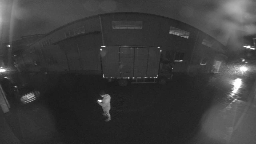
\includegraphics[width=1\textwidth]{Figure/Pretreatment/Img1.png}
\end{minipage}
}
\subfigure[New Image]{
\begin{minipage}[b]{0.46\textwidth}
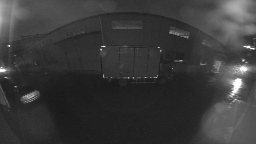
\includegraphics[width=1\textwidth]{Figure/Pretreatment/Img2.png}
\end{minipage}
}
\subfigure[Result]{
\begin{minipage}[b]{0.46\textwidth}
\includegraphics[width=1\textwidth]{Figure/Pretreatment/Result.png}
\end{minipage}
}
\caption{Differential between two images}
\end{figure}

After differential, we need to get the region may include object. And we will use DBSCAN to cluster all region connected.



\subsection{DBSCAN method}
Density-based spatial clustering of applications with noise (DBSCAN) is a density-based clustering algorithm: given a set of points in some space, it groups together points that are closely packed together (points with many nearby neighbors), marking as outliers points that lie alone in low-density regions (whose nearest neighbors are too far away). Before the algorithm, it is necessary to give some definition

\begin{definition}
A point $p$ is a inner point if at least $minPts$ points are within distance $\epsilon$.
\end{definition}
\begin{definition}
A point $q$ is directly reachable from $p$ if point $q$ is within distance $\epsilon$ from point $p$ and $p$ must be a inner point.
\end{definition}
\begin{definition}
A point $q$ is reachable from $p$ if there is a path $p_1, \ldots, p_n $with $p_1 = p$ and $p_n = q$, where each $p_{i+1}$ is directly reachable from $p_i$.
\end{definition}
\begin{definition}
All points not reachable from any other point are outliers.
\end{definition}

For example, as a data set showed in \ref{DBSCAN-Algo}, $A$ is a inner node and $B, C, N$ are outer node. $A, B, C$ are reachable from each other. And we can build a cluster with $A, B$ and $C$. The node $N$ is a noisy node will not join any cluster. 
The processing of cluster for all node in data set has been showed in \ref{DBSCAN-Pros}.

\begin{figure}[H]
\centering
\subfigure[Algorithm]{
\begin{minipage}[b]{0.46\textwidth}
\includegraphics[width=1\textwidth]{Figure/DBSCAN/Algorithm.png}\label{DBSCAN-Algo}
\end{minipage}
}
\subfigure[Cluster method]{
\begin{minipage}[b]{0.46\textwidth}
\includegraphics[width=1\textwidth]{Figure/DBSCAN/Processing.png}\label{DBSCAN-Pros}
\end{minipage}
}
\caption{DBSCAN}
\end{figure}

\begin{figure}[H]
\centering
\subfigure[Differential Image]{
\begin{minipage}[b]{0.46\textwidth}
\includegraphics[width=1\textwidth]{Figure/DBSCAN/InpImg.png}
\end{minipage}
}
\subfigure[Cluster Image]{
\begin{minipage}[b]{0.46\textwidth}
\includegraphics[width=1\textwidth]{Figure/DBSCAN/Result.png}
\end{minipage}
}
\caption{DBSCAN}
\end{figure}

Different from other cluster method, DBSCAN have these advantage:
\\1) Less noisy
\\2) Faster
\\3) Needn't care about the total cluster value



\subsection{Hog Description}
The main processing of Hog Description is 
\begin{algorithm}[H]
\caption{Hog Descriptor}
\begin{algorithmic}
\State Input: $Image[Oriheight][Oriwidth]$
\State STEP1: Down Sample $Image = resize(Image, (height, width))$
\State STEP2: Gamma transform: $Image[i][j] = GammaTable[Image[i][j]]$
\State STEP3: Get the $Gradient$ and $Angle$ image with Sobel operator
\State STEP4: $BlockImgs = [Block\ New\ Image\ with\ BlockX, BlockY, StrideX, StrideY]$
\For {Block in BlockImgs}
\State $Cells = [Get\ the\ Cell\ with\ CellX, CellY in every Block]$
\For {Cell in CellImgs}
\State Statistic Histogram of gradient Hisrogram[nbins]
\State Normalize the Hisrogram
\EndFor
\State Get the $Hog\ descriptor\ in\ the\ Block$
\EndFor
\State Output: $Hog\ descriptor\ of\ the\ image$

\end{algorithmic}
\end{algorithm}

In STEP2 and STEP3, we have

Gamma transform:
\begin{displaymath}
Img_{output} = A\cdot Img_{Input}^{\gamma}
\end{displaymath}

Get gradient and angle:
\begin{displaymath}
SobelX = [-1, 0, 1]\ \ \ \ SobelY = [-1, 0, 1]^{T}
\end{displaymath}
Convolution
\begin{displaymath}
GradientX = Image \ast SobelX
\end{displaymath}
\begin{displaymath}
GradientY = Image \ast SobelY
\end{displaymath}
So we have 
\begin{displaymath}
Gradient = \sqrt{GradientX^2 + GradientY^2}
\end{displaymath}
\begin{displaymath}
Angle = \arctan\left[GradientY \over GradientX\right]
\end{displaymath}


After downsample, the block of image will slide with the method of \ref{slideX} and \ref{slideY}. Then for every block, partial it to some cell as \ref{cell}. Finally statistic the histogram of gradiend in the way of \ref{cellinfo} and \ref{statistic}. Connect all of them, then we can got the Hog feature of a block.


\begin{figure}[H]
\centering
\begin{multicols}{2}
\subfigure[Slide in X]{
\begin{minipage}[b]{0.45\textwidth}
\centering
\includegraphics[width=1\textwidth]{Figure/Hog/BlockX.png}\label{slideX}
\end{minipage}
}
\subfigure[Slide in Y]{
\begin{minipage}[b]{0.45\textwidth}
\centering
\includegraphics[width=1\textwidth]{Figure/Hog/BlockY.png}\label{slideY}
\end{minipage}
}
\end{multicols}


\begin{multicols}{2}
\subfigure[Cells in a block]{
\begin{minipage}[c]{0.45\textwidth}
\centering
\includegraphics[width=1\textwidth]{Figure/Hog/BlockCell.png}\label{cell}
\end{minipage}
}
\subfigure[Cell and statistic]{
\begin{minipage}[c]{0.45\textwidth}
\centering
\includegraphics[width=1\textwidth]{Figure/Hog/Cell.png}\label{cellinfo}
\end{minipage}
}
\end{multicols}


\subfigure[Statistic Data (Color means angle and valus means gradient, statistic of white line area in \ref{cellinfo})]{
\begin{minipage}[b]{0.5\textwidth}
\centering
\includegraphics[width=1\textwidth]{Figure/Hog/Statistic.png}\label{statistic}
\end{minipage}
}

\caption{Hog Block and Cells}
\end{figure}

After Hog description, we can classification feature with SVM. And finally we finished a pedestrain detection processing.
On the one hand, this kind of Hog have to calculate feature of all block in the image. As most block have no human, the most source of calculation have been wasted.
On the other hand, Althrough DNN method have better result and higher accurancy, the model of DNN will be too large for running in a small device which have just 5MB memory.
So to solve this problem, we also changed DBSCAN and Hog with the characteristic of surveillance camera image sequence.





%Section 3============================================================================================
\section{Development of the method}
\subsection{About DBSCAN}
Typically, DBSCAN using the dataset of node. However, as image cluster just have two parameter, x and y. It is not necessary to save all vector which need cluster as a new dataset.

We can list all neighbourhood node as a table in the initial part of the algorithm. And just search the image from the table with DFS(Deep First Search). So the max time complex is $\mathcal{O}{(n\cdot m)}$, where $n$ is total of node which need cluster and $m$ is the size of table. It is faster than original method $\mathcal{O}{(n^2)}$


\subsection{About Hog Descriptor}
Typically, we need several times Hog network with different parameter to determine the location of person.\cite{Lipetski2017} As we used the DBSCAN for object detection, we don't need the whole image description. We just need the descript for every region(Cluster) as a block. This can also make the model of SVM smaller.

\begin{figure}[H]
\centering
\subfigure[]{
\begin{minipage}[b]{0.45\textwidth}
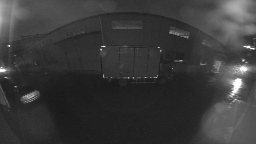
\includegraphics[width=0.45\textheight]{Figure/Pretreatment/Img2.png}
\end{minipage}
}

\begin{multicols}{4}
\subfigure[]{
\begin{minipage}[b]{0.1\textwidth}
\includegraphics[width=1\textwidth]{Figure/Development/1.png}
\end{minipage}
}
\\
\subfigure[]{
\begin{minipage}[b]{0.1\textwidth}
\includegraphics[width=1\textwidth]{Figure/Development/2.png}
\end{minipage}
}
\\
\subfigure[]{
\begin{minipage}[b]{0.1\textwidth}
\includegraphics[width=1\textwidth]{Figure/Development/3.png}
\end{minipage}
}
\\
\subfigure[]{
\begin{minipage}[b]{0.1\textwidth}
\includegraphics[width=1\textwidth]{Figure/Development/4.png}
\end{minipage}
}
\end{multicols}

\caption{Image and Cluster image}
\end{figure}


Result:\\
a: $0.268041, 0.028966, 0.259261, \ldots, 0.004802, 0.104433, length = 144$\\
b: $0.436385, 0.008739, 0.054215, \ldots, 0.021862, 0.255745, length = 144$\\
c: $0.259077, 0.057242, 0.074549, \ldots, 0.009185, 0.243987, length = 144$\\
d: $0.349008, 0.100296, 0.149541, \ldots, 0.007501, 0.184265, length = 144$\\[2ex]
All Image: $2.26329e^{-11}, 2.595552e^{-11}, 1.03369275e^{-11}, \ldots, 2.8235041e^{-11}, 1.8345979e^{-10}, \\length = 3888$



%Section 4============================================================================================
\section{About IFECP Dataset(Infrared Fish Eye Camera Pedestrian Dataset)}





%Section 5============================================================================================
\section{Result}
\begin{figure}[H]
\begin{multicols}{2}
\centering
\subfigure[Result 1]{
\begin{minipage}[b]{0.45\textwidth}
\centering
\includegraphics[width=1\textwidth]{Figure/PRWResult/1.png}
\end{minipage}
}

\subfigure[Result 2]{
\begin{minipage}[b]{0.45\textwidth}
\centering
\includegraphics[width=1\textwidth]{Figure/PRWResult/2.png}
\end{minipage}
}
\\
\subfigure[Result 3]{
\begin{minipage}[b]{0.45\textwidth}
\centering
\includegraphics[width=1\textwidth]{Figure/PRWResult/3.png}
\end{minipage}
}

\subfigure[Result 4]{
\begin{minipage}[b]{0.45\textwidth}
\centering
\includegraphics[width=1\textwidth]{Figure/PRWResult/4.png}
\end{minipage}
}
\end{multicols}
\caption{Result (PRW Dataset)}
\end{figure}





%Section 6============================================================================================
\section{Acknowledge}





%Section 7============================================================================================
\section{Appendix}





%Reference============================================================================================
\newpage
\medskip
\bibliographystyle{plain}
\bibliography{/Users/kazukiamakawa/Desktop/お仕事関連/Paper/KazukiAmakawa.bib}

\end{document}
%~~~~~~~~~~~~~~~~~~~~~~~~~~~~~~~~~~~~~~~~~~~~~~~~~~~~~~~~~~~~~~~~~~~~~~~~~~~~~~~~~~~~~~~~~~~~~~~~~~~~~


%Sample Codes
\begin{definition}
Ring\\

\end{definition}


\begin{table}[!htb]
\centering  
\caption{Instruction}  
\begin{tabular}{|c|c|c|c|c|}
\hline
1 & 2   & $+, \cdot$ & 0,1   & 3\\
\hline
4 & 5 & 6     & 7 & 8 \\  
\hline
\end{tabular}  
\end{table}  


\noindent\rule[0.25\baselineskip]{\textwidth}{1pt}
\begin{lstlisting}[language = Matlab][basicstyle=\ttfamily][!htb]
[Code: Matlab]
clear
[number, txt, raw] = xlsread('File');
\end{lstlisting} 
\noindent\rule[0.25\baselineskip]{\textwidth}{1pt}


\begin{figure}[H]
\begin{center}
\includegraphics[width=1.00\textwidth]{Figure/MLResult.png} \\
图3 CARLA算法的迭代情况\\
\end{center}
\end{figure}


\begin{algorithm}[H]
\caption{CARLA algorithm main steps}
\begin{algorithmic}
1)
\end{algorithmic}
\end{algorithm}


\begin{flalign}
& & \nonumber\\
& & \nonumber
\end{flalign}